\vspace{-2pt}
\section{Impact of energy savings on user performance}
\label{sec:evaluation-energy_savings}
\vspace{-4pt}

%As mentioned before in Section~\ref{sec:introduction}, 
The main goal of energy saving strategies is to minimize the energy consumption while ensuring no impact on the Quality of Experience of end-users.
MNOs employ several metrics and approaches to quantify service quality, ranging from end-users reporting anomalies to user equipment testing devices deployed across the country and server-end KPIs. 
We focus here on an objective metric --the average user throughput at the cell level-- which is an average estimation of the throughput served to UEs by a specific cell. 
The question we aim to answer in this section is: when a capacity cell enters into sleep mode, are the \textit{fallback cells} (i.e., the active cells that receive the load previously accommodated by the now sleeping capacity cell) able to deliver a good service performance?

\vspace{-2pt}
\subsection{Characterizing post-sleep handovers}
\vspace{-2pt}

%In order to measure this impact, it is necessary first to define what we meant by \textit{fallback cells}. 
Related work~\cite{celebi2019load, shahid2020load, teng2021joint} assumes that when the capacity cell enters into the energy saving mode and slowly decreases, the emitting power causes the UE to trigger a detach and attach to a specific cell that also fully overlaps the area of the capacity cell. In practice, this is a far more complex phenomenon, and UEs attach to a variety of nearby cells.  

We propose a data-driven approach to gain insights into these transitions, and rely on the detach and attach events using logs from the MME that we captured during the trials. 
%In order to understand this phenomenon better and obtain insight, we ran a set of measurements that focused on the detach and attach events using logs from the MME.
We use the following methodology: 
\begin{itemize}[leftmargin=*]
    \item Given the set of capacity cells and the specific time with 1-second resolution, when the cell sleep mode is activated: ${(C_i, [t_1, t_2, ..., t_n])}$.
    \item For each capacity cell $C_i$ and for each time instance $t_i$, we obtain the set of UEs $[\text{UE}_1, \text{UE}_2, ..., \text{UE}_m]$ whose last service request was served by $C_i$ inside the time windows $(t_i - \delta_{start},  t_i]$. This time window is in place to ensure that the interaction was recent.
    \item Next, we identify the cells $F$ where the UEs are attached to during the time windows $(t_i, t_i + \delta_{end}]$. 
    \item Finally, we obtain a set of tuple ${(C_i, t_i, \text{UE}_k, F_l)}$ that represents that the $\text{UE}_k$ was attached to capacity cell $C_i$ and when this enters into sleep mode, reattached from it, and attach to a \textit{fallback cell} $F_l$.
\end{itemize}
We tested different values for $\delta_{start}$ and $\delta_{end}$ for one day of experimentation. Empirical results showed that using a symmetric window $\delta_{start} = \delta_{end} = 30\text{min}$ provided a good trade-off to ensure that the transfer was due to the activation of the sleeping mode and that the number of samples collected is sufficient.
With this, we collect the final measurements in the two trial regions for more than one week, and obtained more than $81,000$ transfer tuples. 

These results show that $40\%$ of the transfers in the Dense region and $44\%$ in the Sparse region occur to relatively nearby cells located in other cell sites (within $1.8$km and $3.9$km, respectively; note that these distances vary in function of the cell deployment and density).
Conversely, $60\%$ and $56\%$ of the attachments happen to active cells in the same site as the capacity cell $C_i$, of which around $80\%$ of these happen to cells in the same sector. 
Although more than $40\%$ of the transfers happen to other base stations, they are geographically sparse, meaning that the UEs spread across these cells and their density decays with the increase in distance.
%; a single of these cells does not receive a major portion of the UEs.
Meanwhile, the cells in the same sector as the capacity cell provide service to a more cohesive group of UEs, which may affect network performance. Therefore, we focus on these cells, which we refer to as the \textit{fallback cells} in the rest of the paper.

% we can now inspect the change in the average user throughput and cell utilization in order to disambiguate the case when the throughput decrease may be caused by low utilization or the lack of resources.

\vspace{-2pt}
\subsection{Quantifying critical cell sleep decisions}
\vspace{-2pt}

Our objective is to identify  \textit{fallback cells} that were adversely affected by the UEs transfer after cell sleep events, \ie by a critical decrease in their offered user average throughput.
In order to ensure that the user average throughput decrease was related to an increase in demand, we also analyzed the \textit{fallback cell} utilization to disambiguate the cases where the throughput can decay because of low resource utilization (\eg by users with little traffic demands) or due to the impact of the new UEs absorbed by the cell.

% were having a previous state of high utilization and user throughput before the $C^i$ activated the cell sleep mode and after $t_i$ transitioned to a state of high utilization but poor user throughput. \ael{this sentence makes no sense to me, please re-write this @ORLANDO, I dunno what you meant here}
Figure~\ref{fig:tti_utilization_user_throughput} shows how the Transmission Time Interval (TTI) utilization --which, similarly to PRB utilization, is a proxy for the level of saturation of a cell-- and user average throughput are related; each sample corresponds to one \textit{fallback cell}, for which we report the two metrics above in the aftermath of a sleep event of a capacity cell in the same site and sector.
We then define two thresholds that allow distinguishing between normal/low user throughput and normal/high cell utilization.
For TTI utilization the threshold is set at $45\%$ (horizontal line in Figure~\ref{fig:tti_utilization_user_throughput}) based on the third quartile of the TTI utilization distribution over the full period of the trials; the average user throughput is considered low below $8\text{Mbps}$ (vertical line in the figure), based on literature analysis, private communications with the operations teams, and statistical analysis of the empirical throughput distribution. 
%Note that this value doesn't mean that the user is having a poor experience; instead, it reflects the fact that the QoE is lower than expectations. 
Note that these thresholds do indicate non-operational conditions that would trigger an urgent intervention by the MNO but are symptomatic of a significant degradation of the end-user experience.

\begin{figure}[!t]
    \centering
    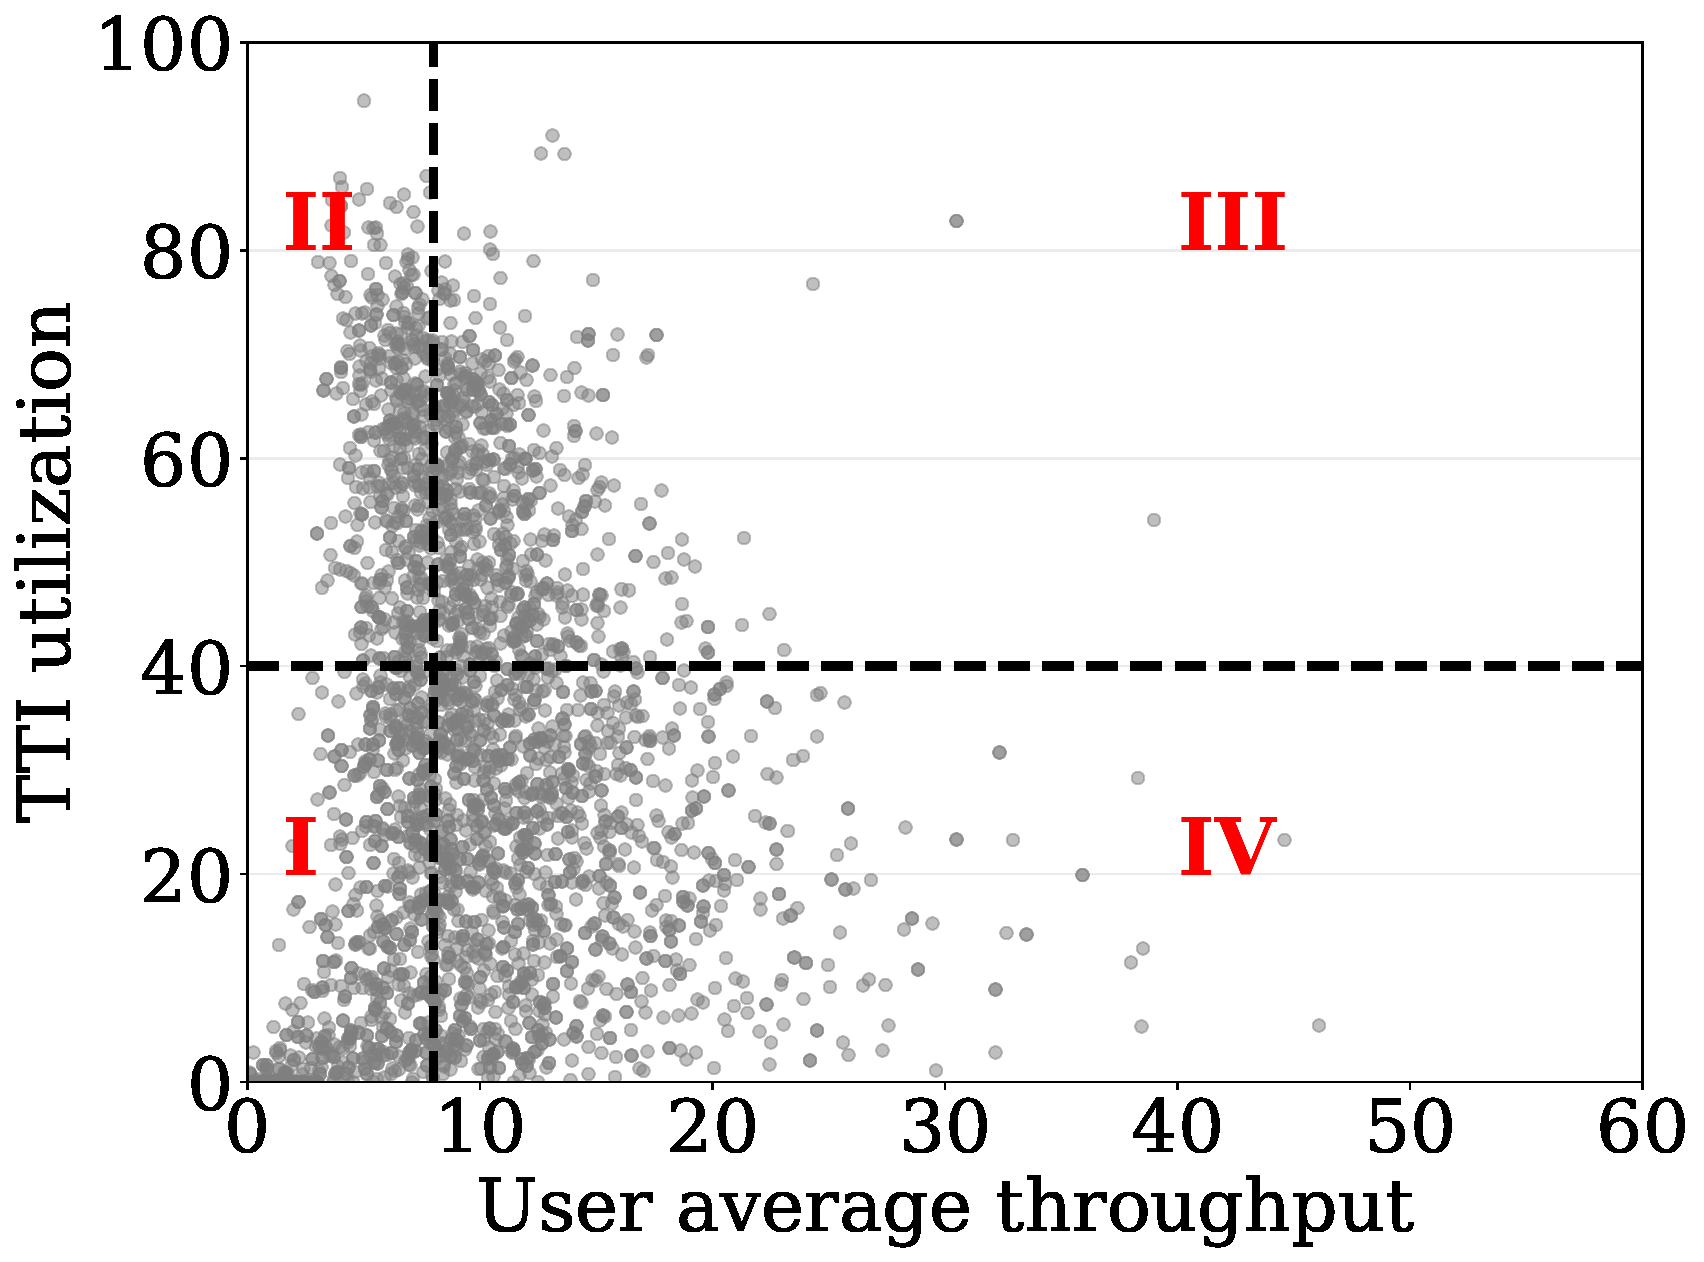
\includegraphics[width=.65\columnwidth]{images/kpi/scatter_throughput_utilization/north_london_Baseline_after_grey.pdf}
    \vspace{-4pt}
    \caption{\small TTI utilization and user average throughput of fallback cells instants before the corresponding capacity cell enters into sleep mode. 
    % \mf{explain the meaning of each quadrant and associate `names' to them, \ie the important thing is introducing the notion of `normal', `recover', etc.}
    % \mf{make the roman number more evident if those are used in the text; also you may want to rasterize the image}
    %\js{is it TTI or PRB utilization? Change the caption and Y label accordingly}
    \label{fig:tti_utilization_user_throughput}}
    \vspace{-15pt}
\end{figure}

\begin{figure*}[!t]
    \centering
    \subfloat[Night-loose]{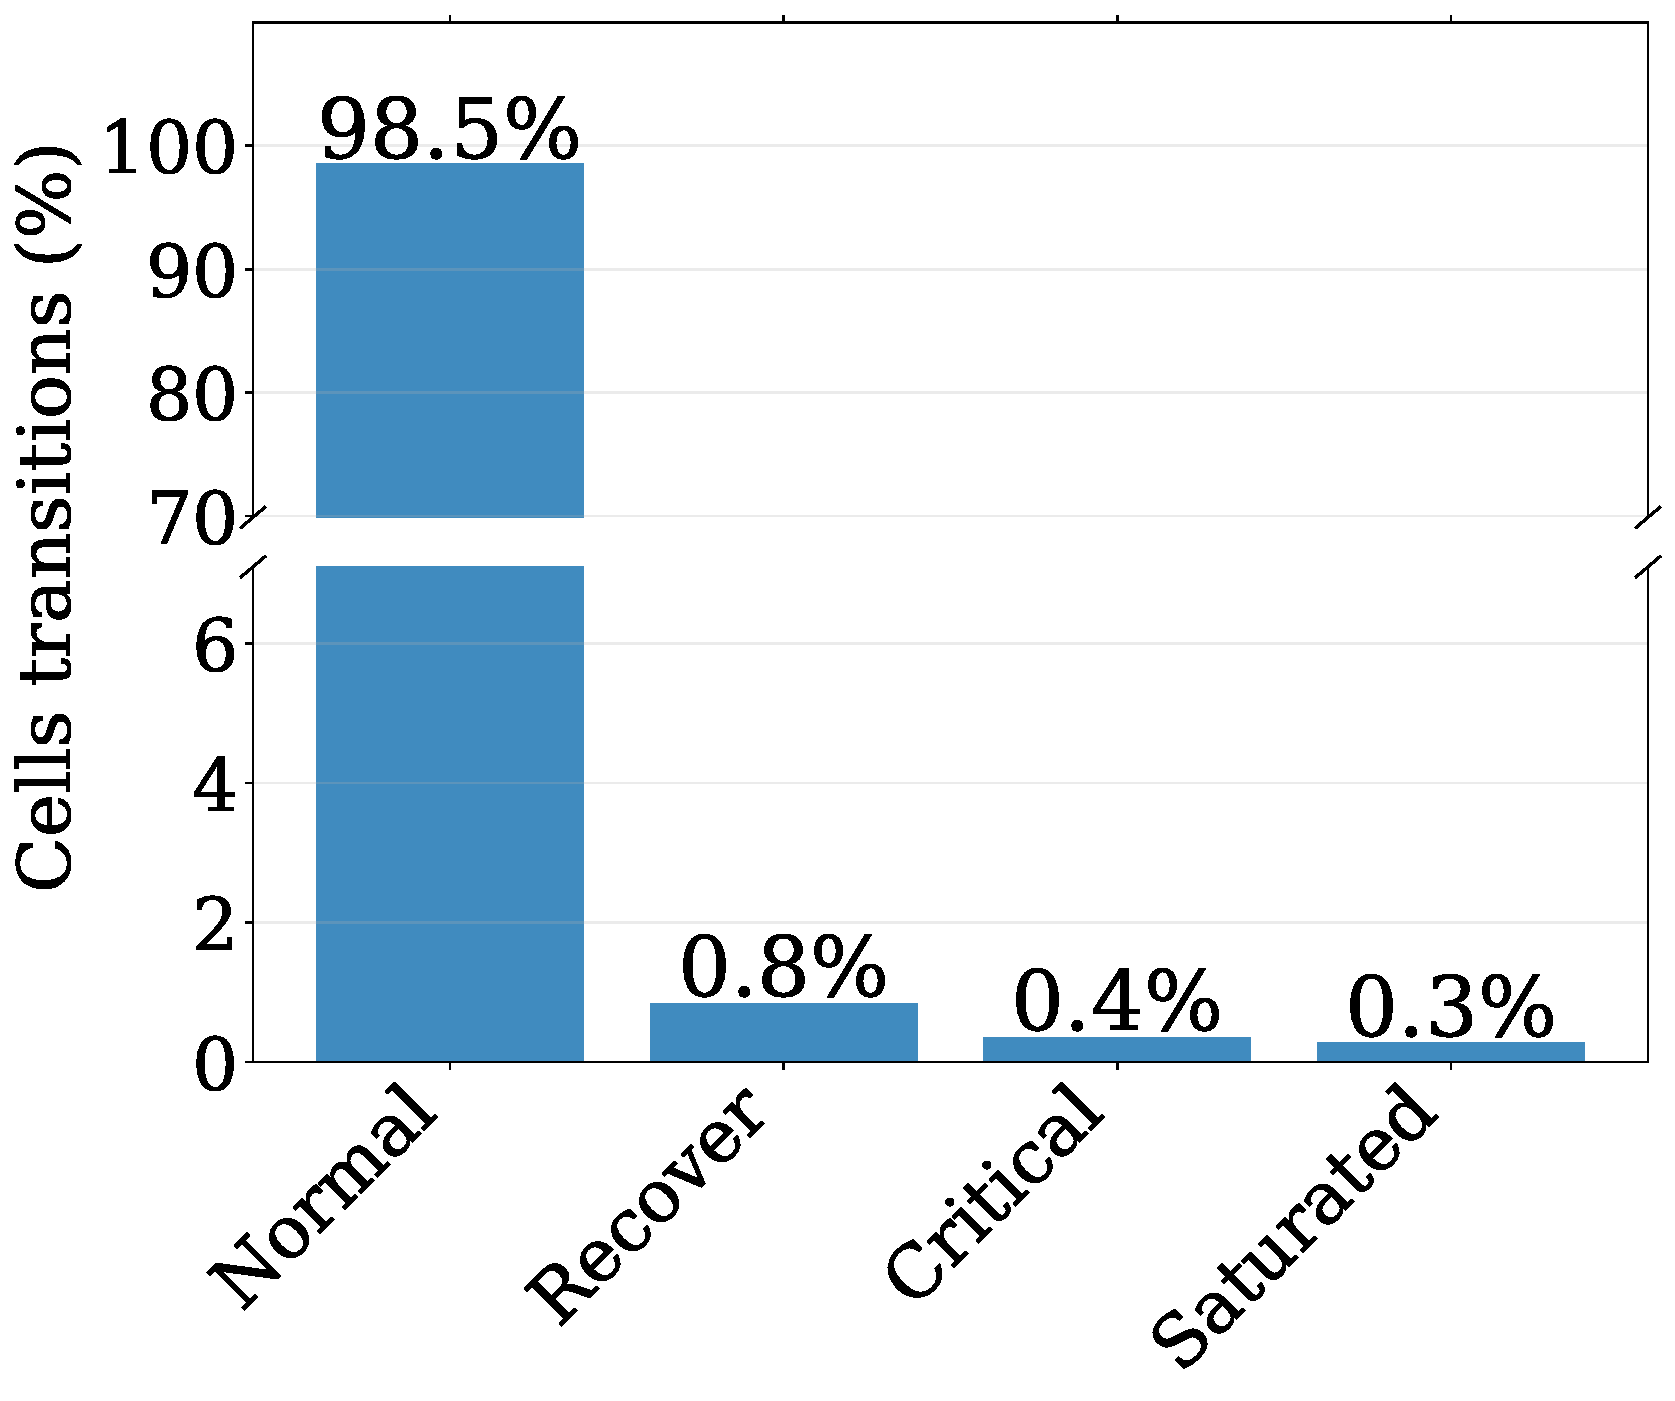
\includegraphics[width=.2\textwidth]{images/kpi/impact_classes/events_per_class_area_merge_11_6.pdf}}
    \subfloat[Night-strict]{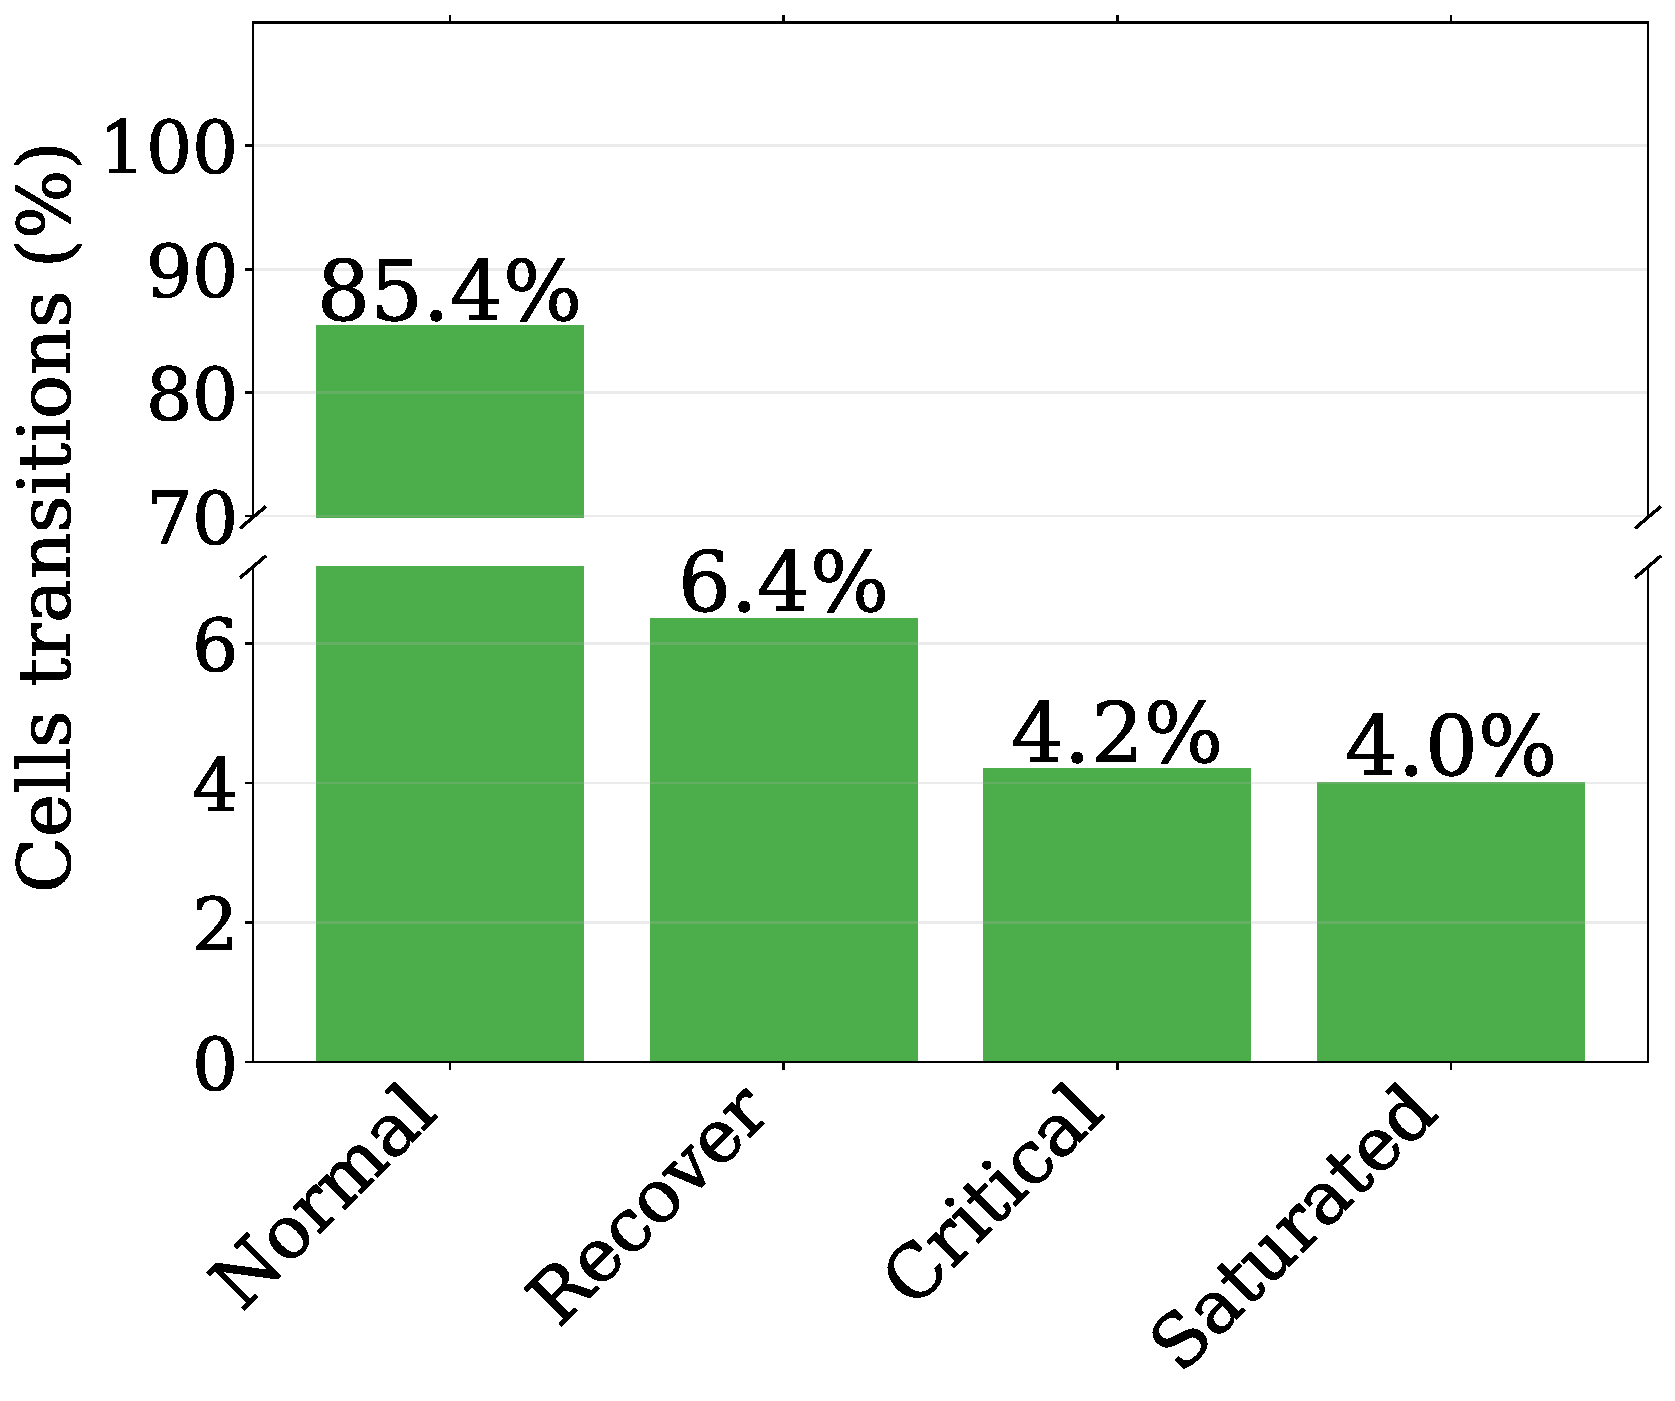
\includegraphics[width=.2\textwidth]{images/kpi/impact_classes/events_per_class_area_merge_Baseline.pdf}}
    \subfloat[Full-loose]{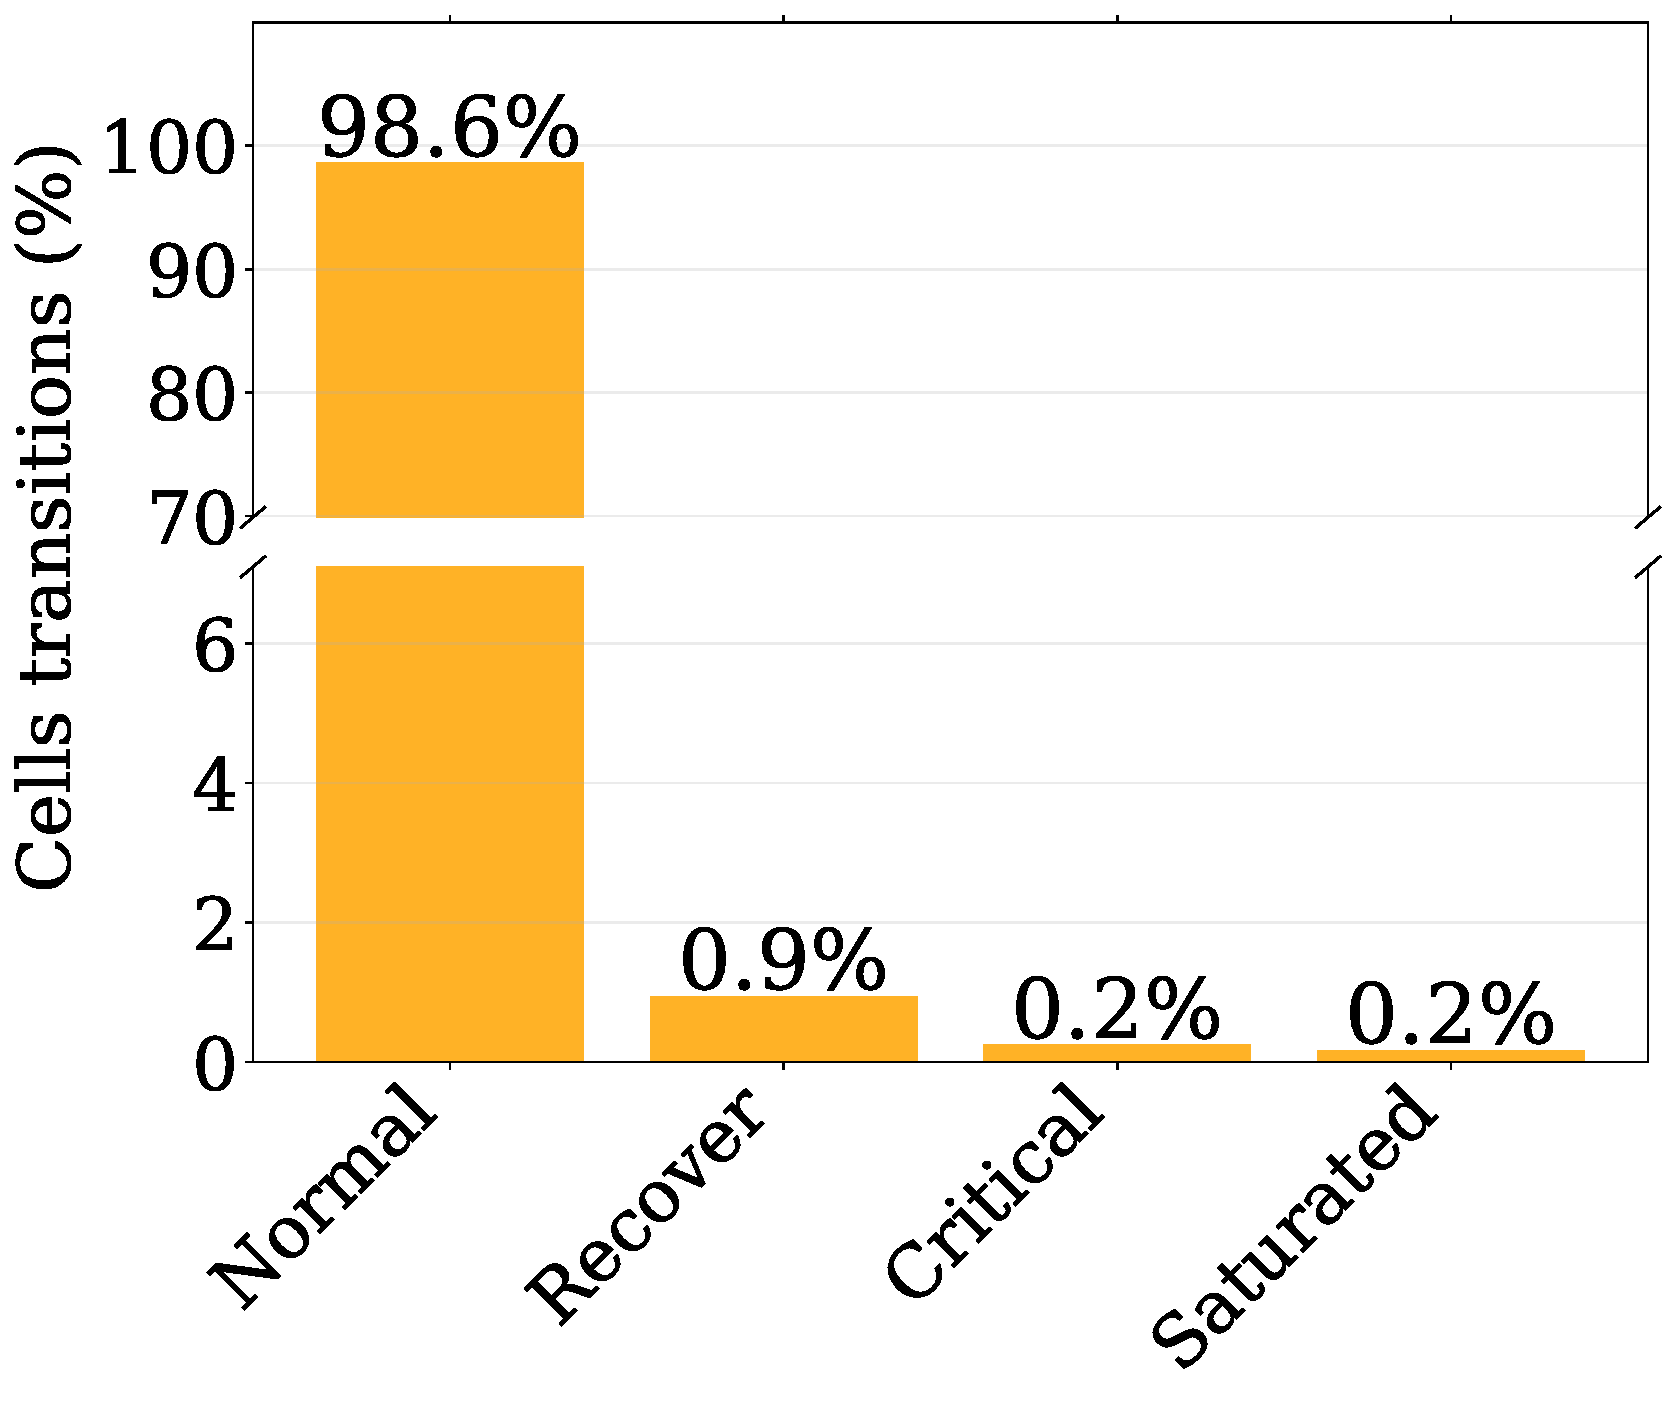
\includegraphics[width=.2\textwidth]{images/kpi/impact_classes/events_per_class_area_merge_24x7_1.pdf}}
    \subfloat[Full-moderate]{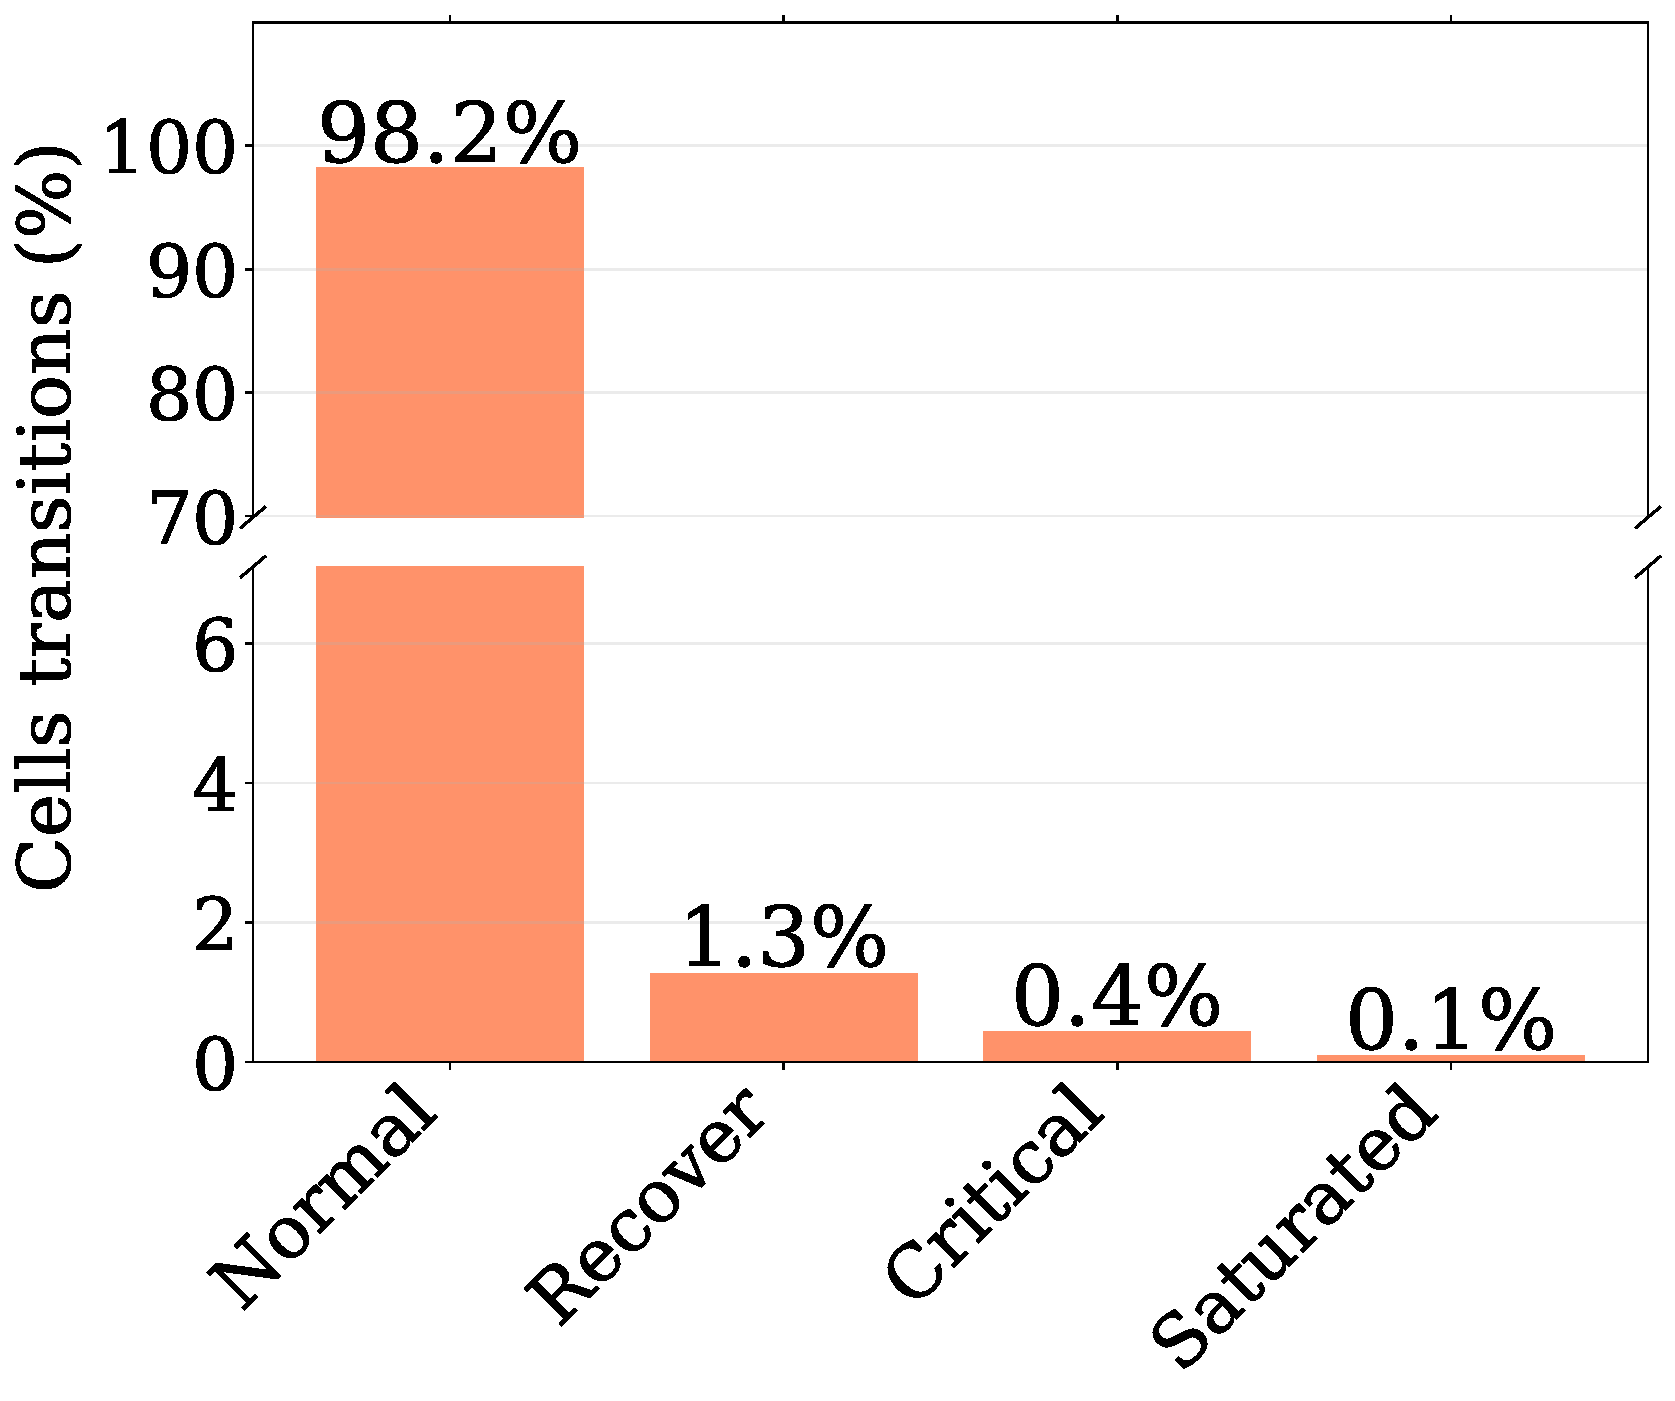
\includegraphics[width=.2\textwidth]{images/kpi/impact_classes/events_per_class_area_merge_24x7_2.pdf}}
    \subfloat[Full-strict]{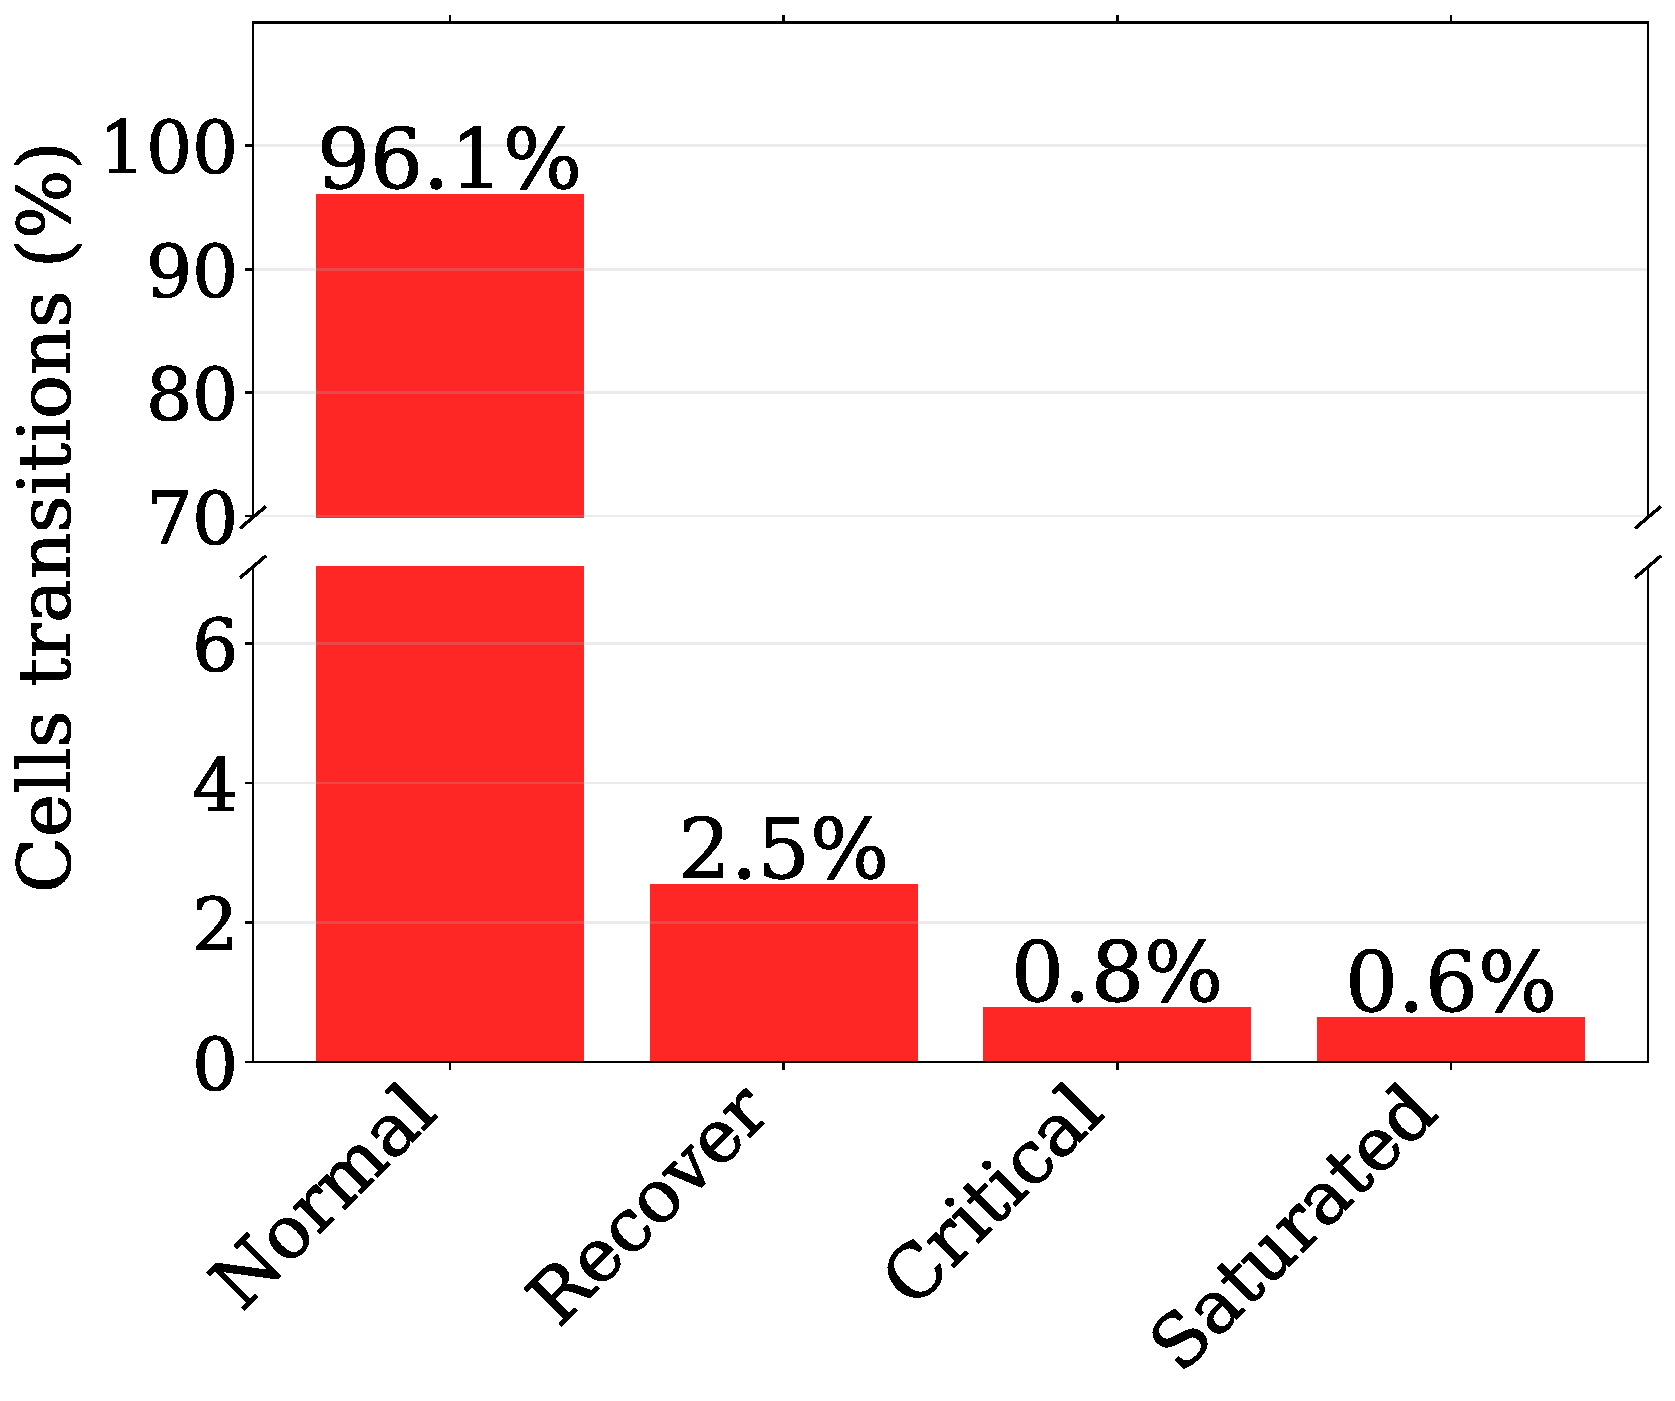
\includegraphics[width=.2\textwidth]{images/kpi/impact_classes/events_per_class_area_merge_24x7_3.pdf}}
    \vspace{-4pt}
    \caption{\small Cells transition percentage, for each strategy. Regions were aggregated due to their similar values.
    % \mf{`break' the y axis at 7, not at 12}
    \label{fig:events_per_class}}
    \vspace*{-10pt}
\end{figure*}


Using these thresholds, we can define four quadrants in Figure~\ref{fig:tti_utilization_user_throughput}: I) low user average throughput and low utilization, II) low average user throughput and high utilization, III) within range user throughput and high utilization, and IV) within range user throughput and low utilization.
Based on the transition between states on the \textit{fallback cells} before and after the corresponding capacity cells enter into sleep mode, they can be classified into these four transition classes: 
\begin{itemize}[leftmargin=*]
    \item \textbf{Critical}: The \textit{fallback cell} average user throughput was within the expected values, but after the capacity cells sleep, it is lower than the 8Mbps threshold while the utilization increases (\ie quadrants I, III, and IV $\rightarrow$ quadrant II).
    \item \textbf{Saturate}: The \textit{fallback cell} had below the threshold user throughput and high utilization and remained in this state after the capacity cells went to sleep (\ie quadrant II $\rightarrow$ quadrant II).
    \item \textbf{Recovery}: The \textit{fallback cell} experiences below the threshold user average throughput and high utilization, but after the capacity cell go to sleep, the user average throughput is within the expected range (\ie quadrant II $\rightarrow$ quadrants I, III or IV).
    \item \textbf{Normal}: All the cases where the \textit{fallback cell} user's average throughput remains within the expected range before and after the capacity cells sleep, indicating no impact.
\end{itemize}



%Our next step was to quantify how often these transition classes appear across the different strategies. 
With this, Figure~\ref{fig:events_per_class} shows the percentage of times that we categorized the \textit{fallback cells} in a transaction class. 
We find that ($i$) all policies generate all four situations in similar fractions and ($ii$) the fractions of `critical' and `saturated' cells do not grow significantly with the aggressiveness of the policy.

% \begin{figure}
%     \centering
%     \subfloat{
%         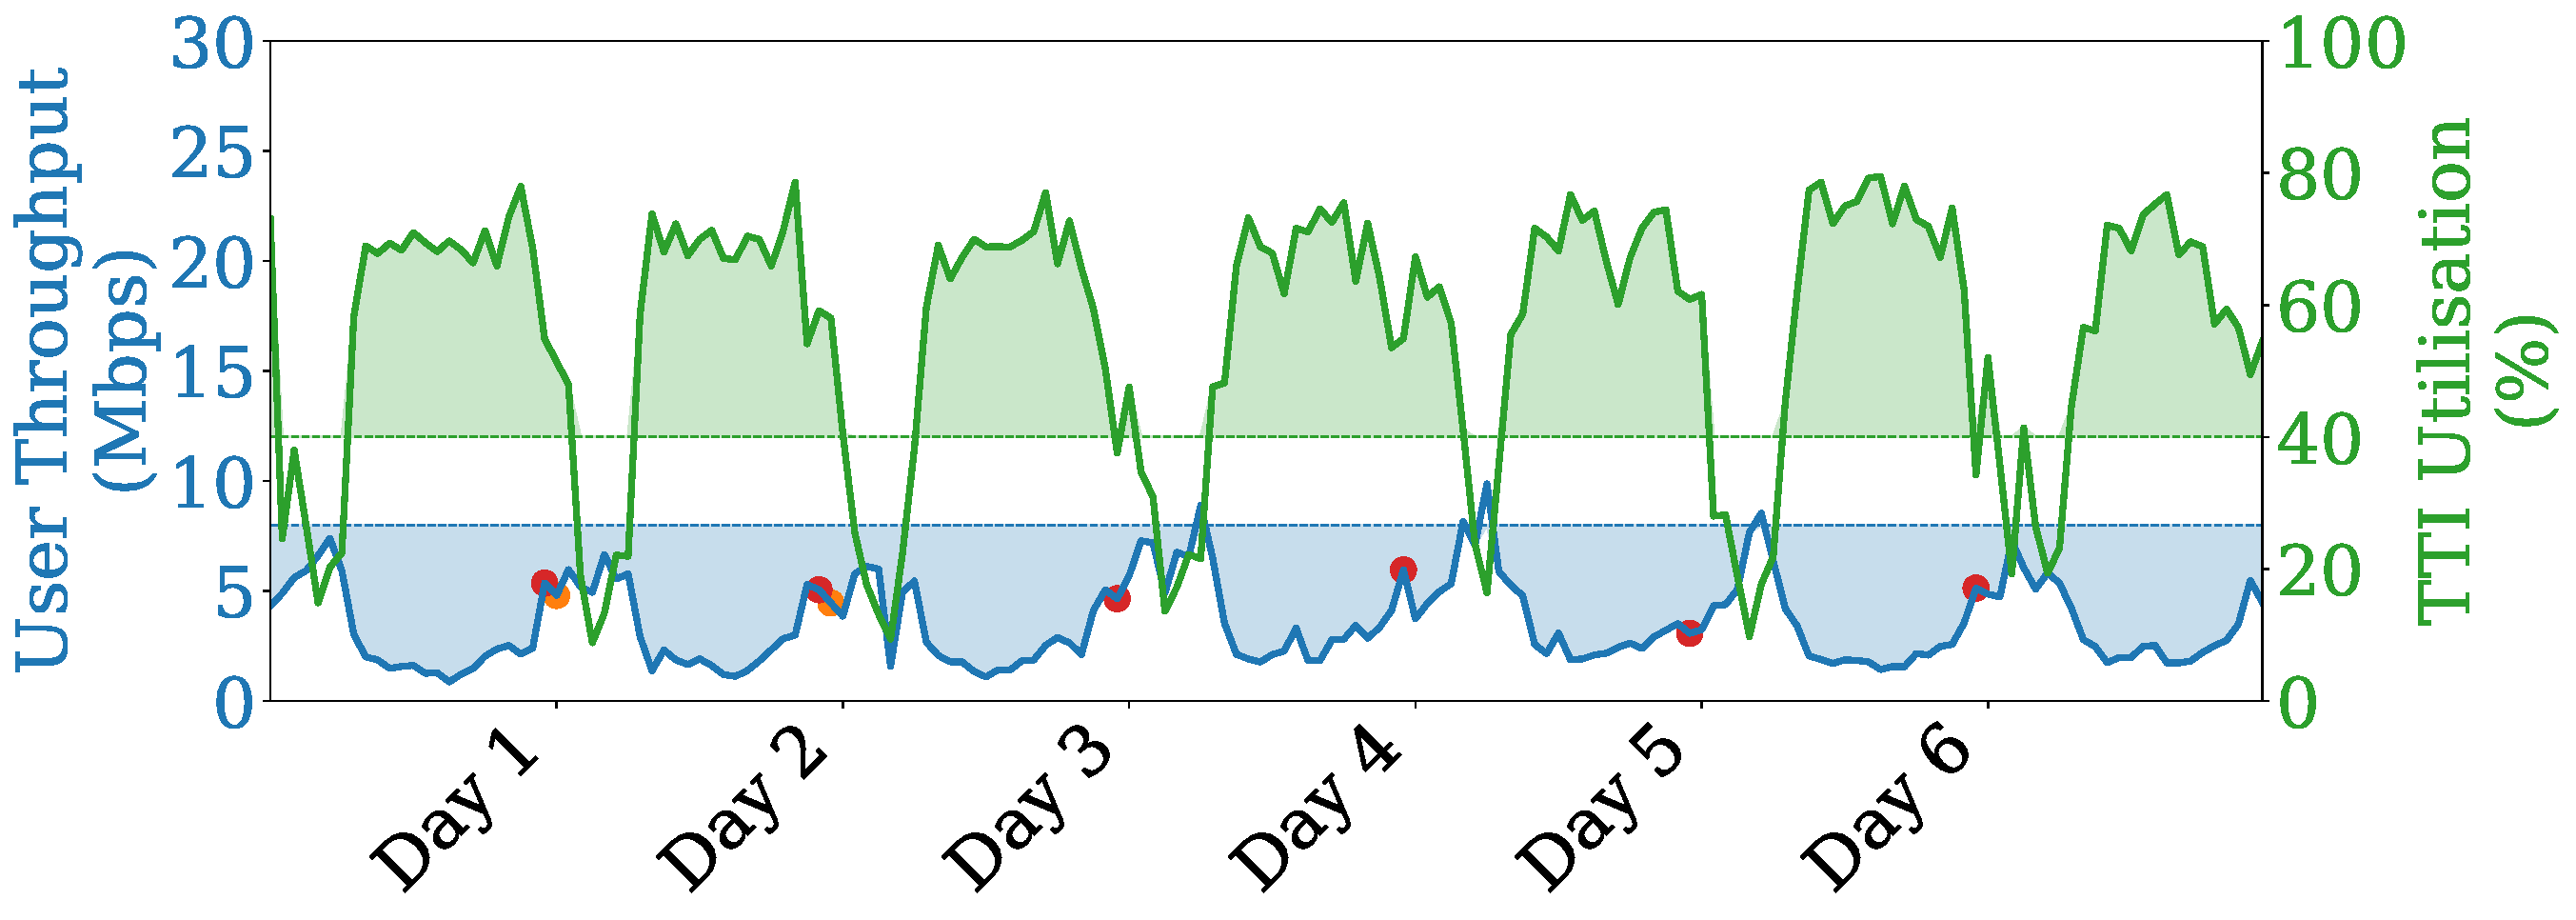
\includegraphics[width=.85\columnwidth]{images/kpi/qualitative_examples/southeast/120-503723_Baseline.pdf}}
        
%     \subfloat{
%         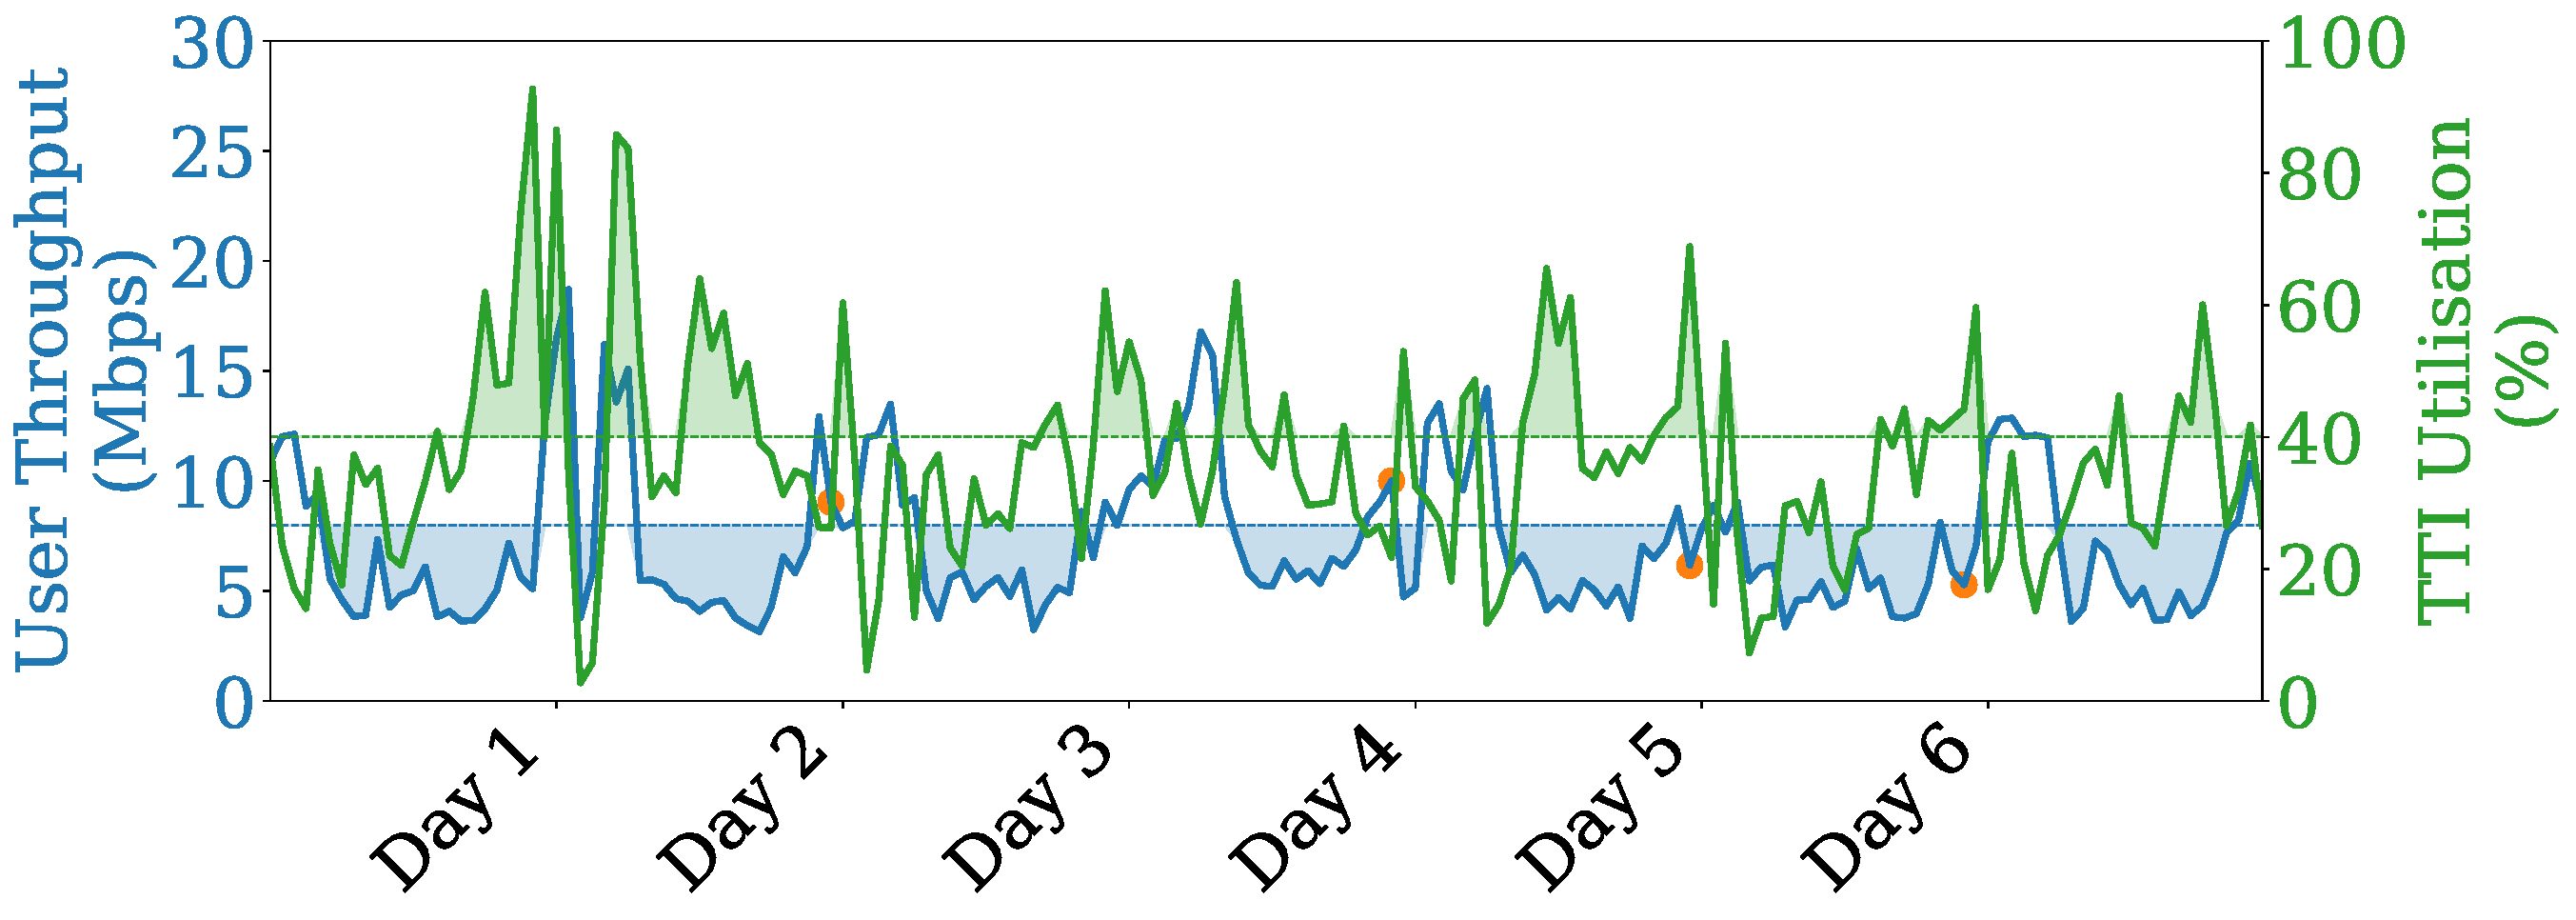
\includegraphics[width=.85\columnwidth]{images/kpi/qualitative_examples/southeast/130-504047_11_6.pdf}
%     }
%     \caption{Time series of user average throughput and TTI Utilization on fallback antennas, highlighting the moments when corresponding capacity booster enters into cell sleep mode.}
%     \label{fig:qualitative_examples_fallback_antennas}
% \end{figure}

% Figure~\ref{fig:qualitative_examples_fallback_antennas} show the user average throughput and utilization for one the \textit{fallback antennas} and highlight the moments where the corresponding capacity booster enter into sleep mode. 

\begin{figure*}
    \centering
    \subfloat{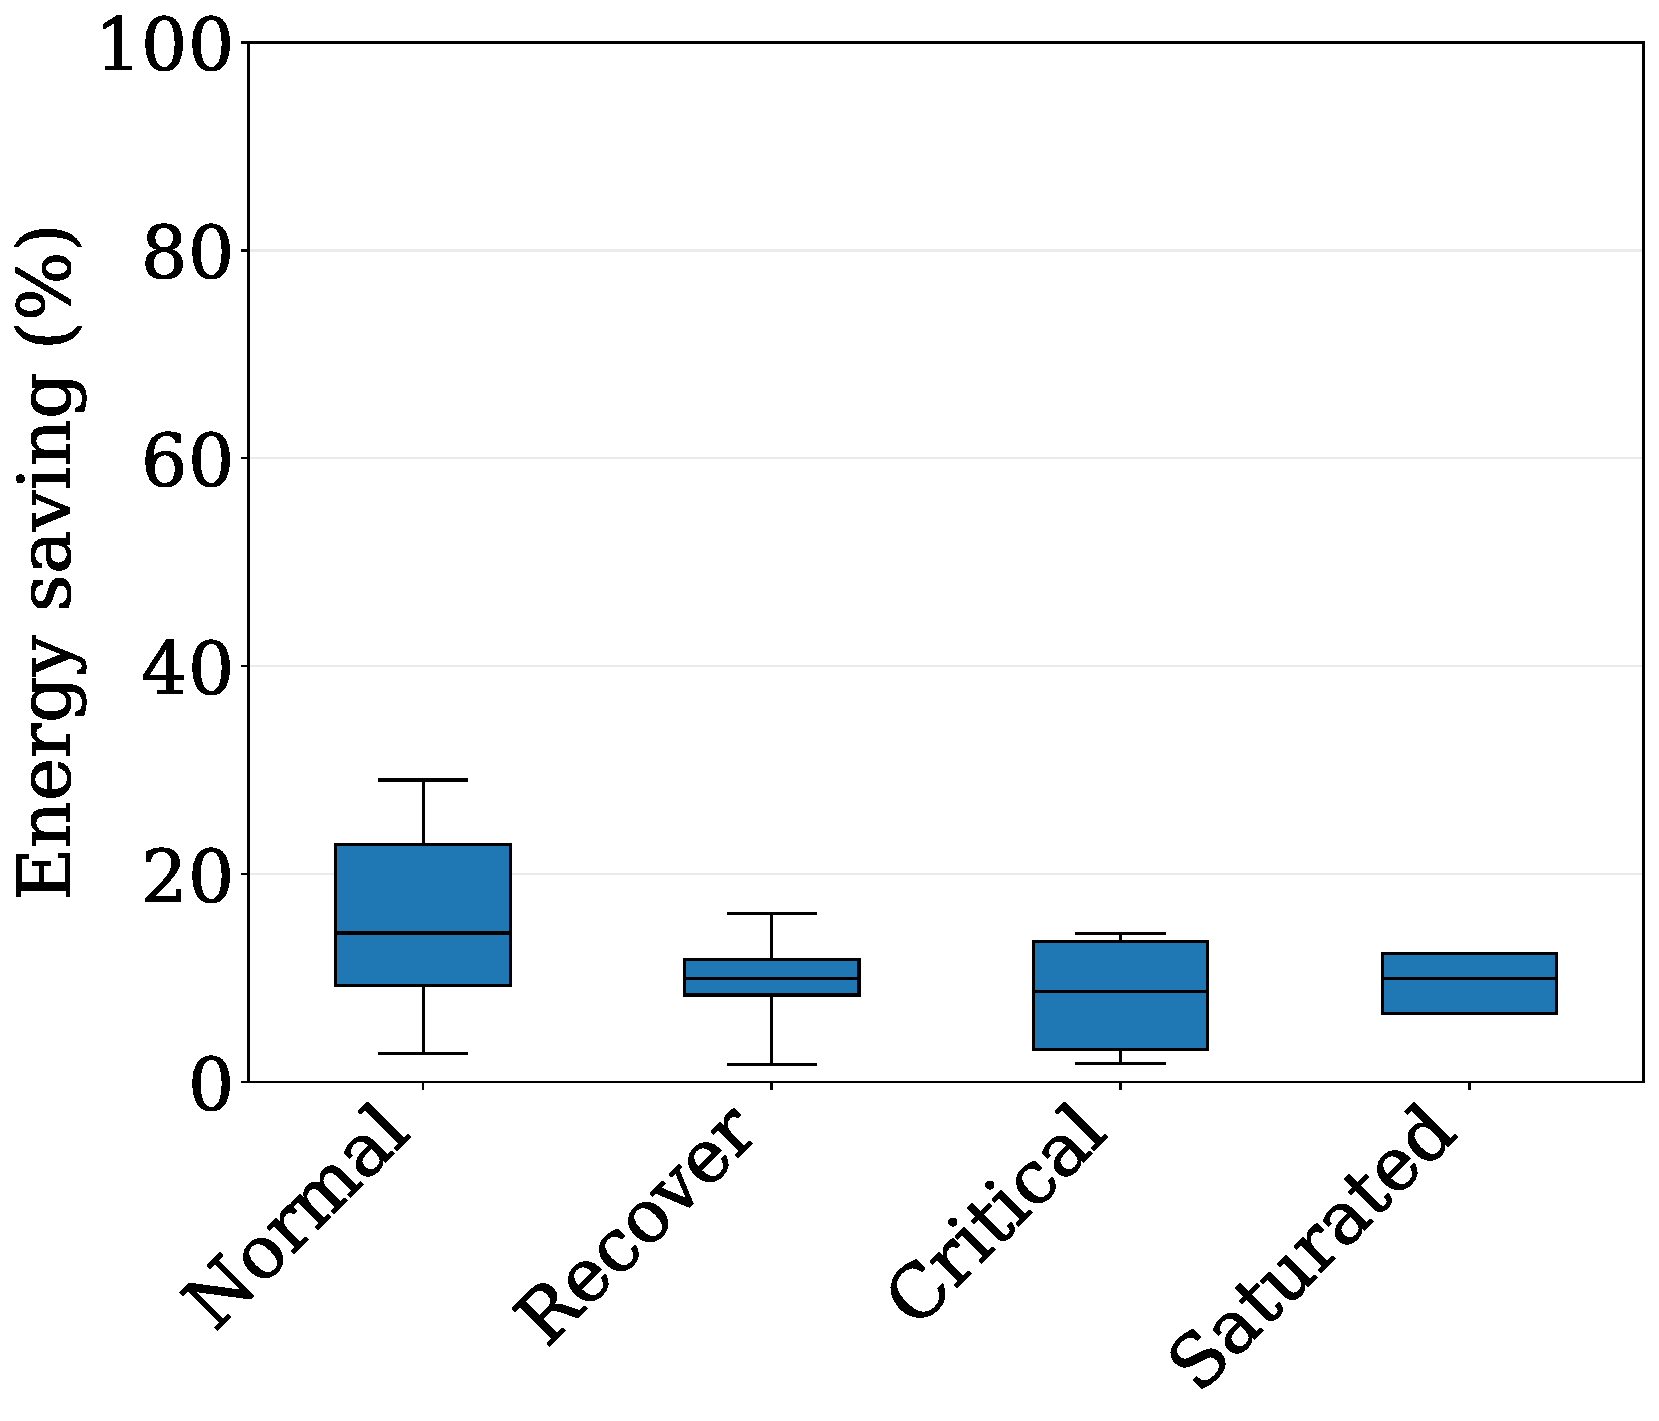
\includegraphics[width=.2\textwidth,trim={0 160pt 0 0},clip]{images/kpi/saving_per_class/north_london/energy_saving_class_11_6.pdf}}
    \subfloat{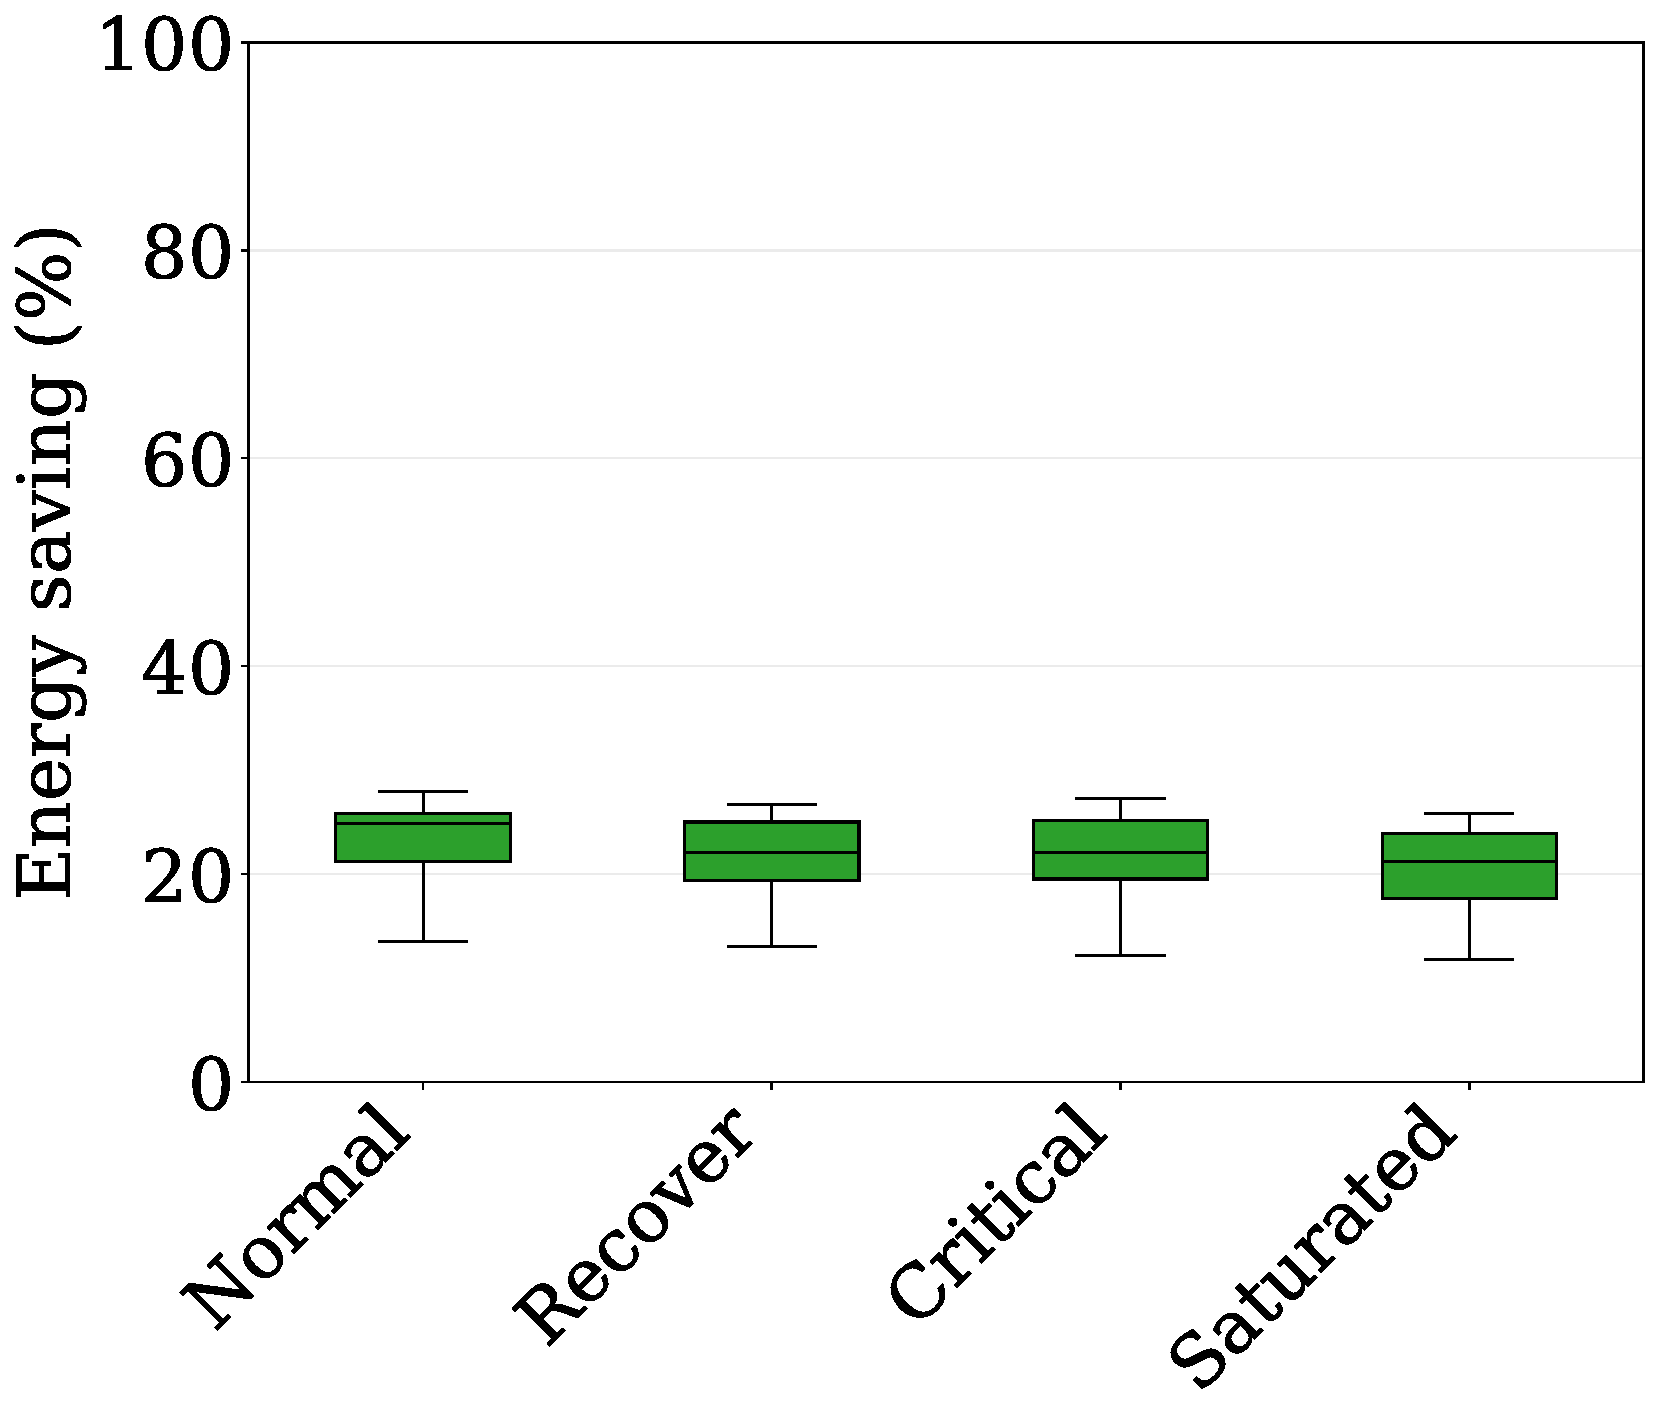
\includegraphics[width=.2\textwidth,trim={0 160pt 0 0},clip]{images/kpi/saving_per_class/north_london/energy_saving_class_Baseline.pdf}}
    \subfloat{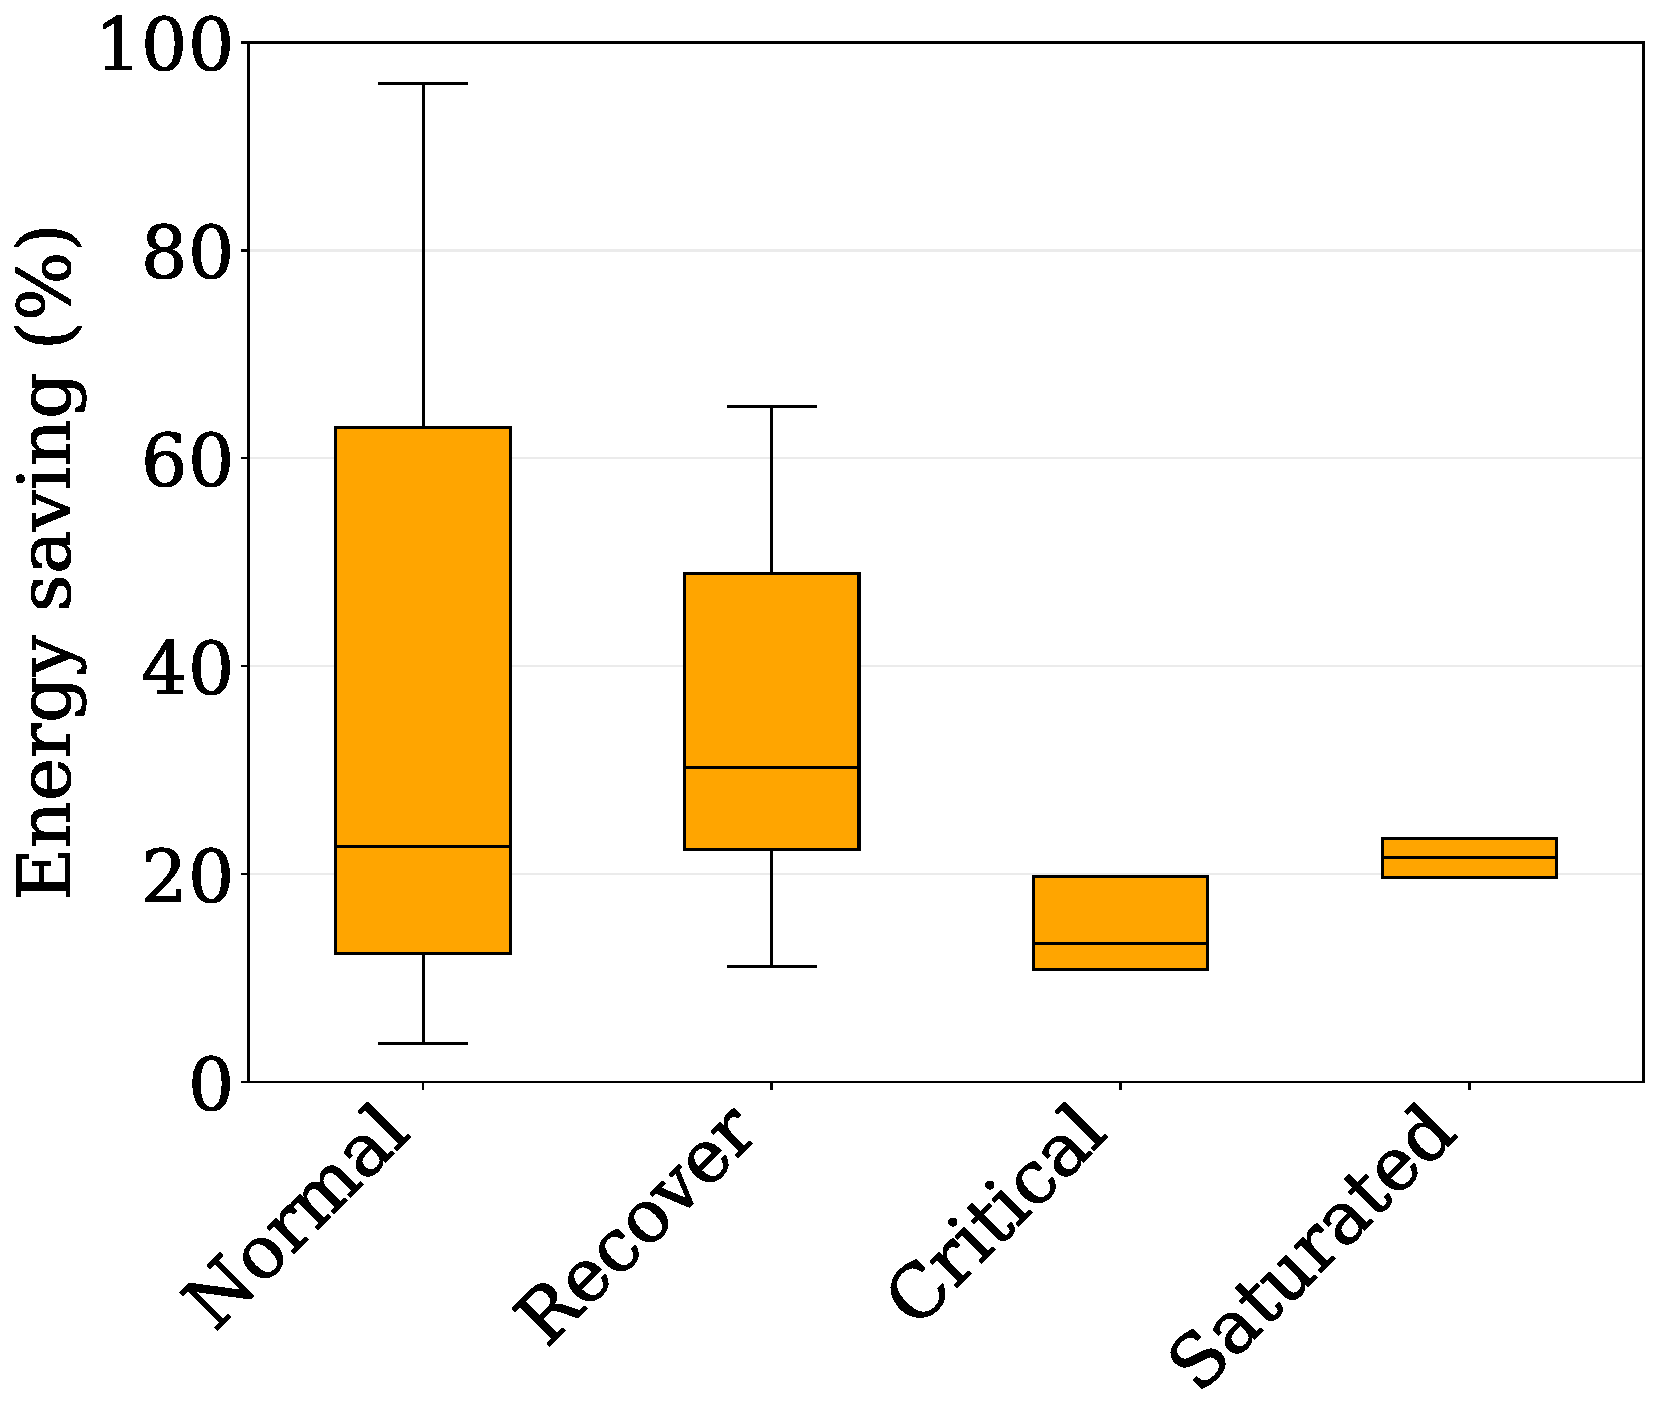
\includegraphics[width=.2\textwidth,trim={0 160pt 0 0},clip]{images/kpi/saving_per_class/north_london/energy_saving_class_24x7_1.pdf}}
    \subfloat{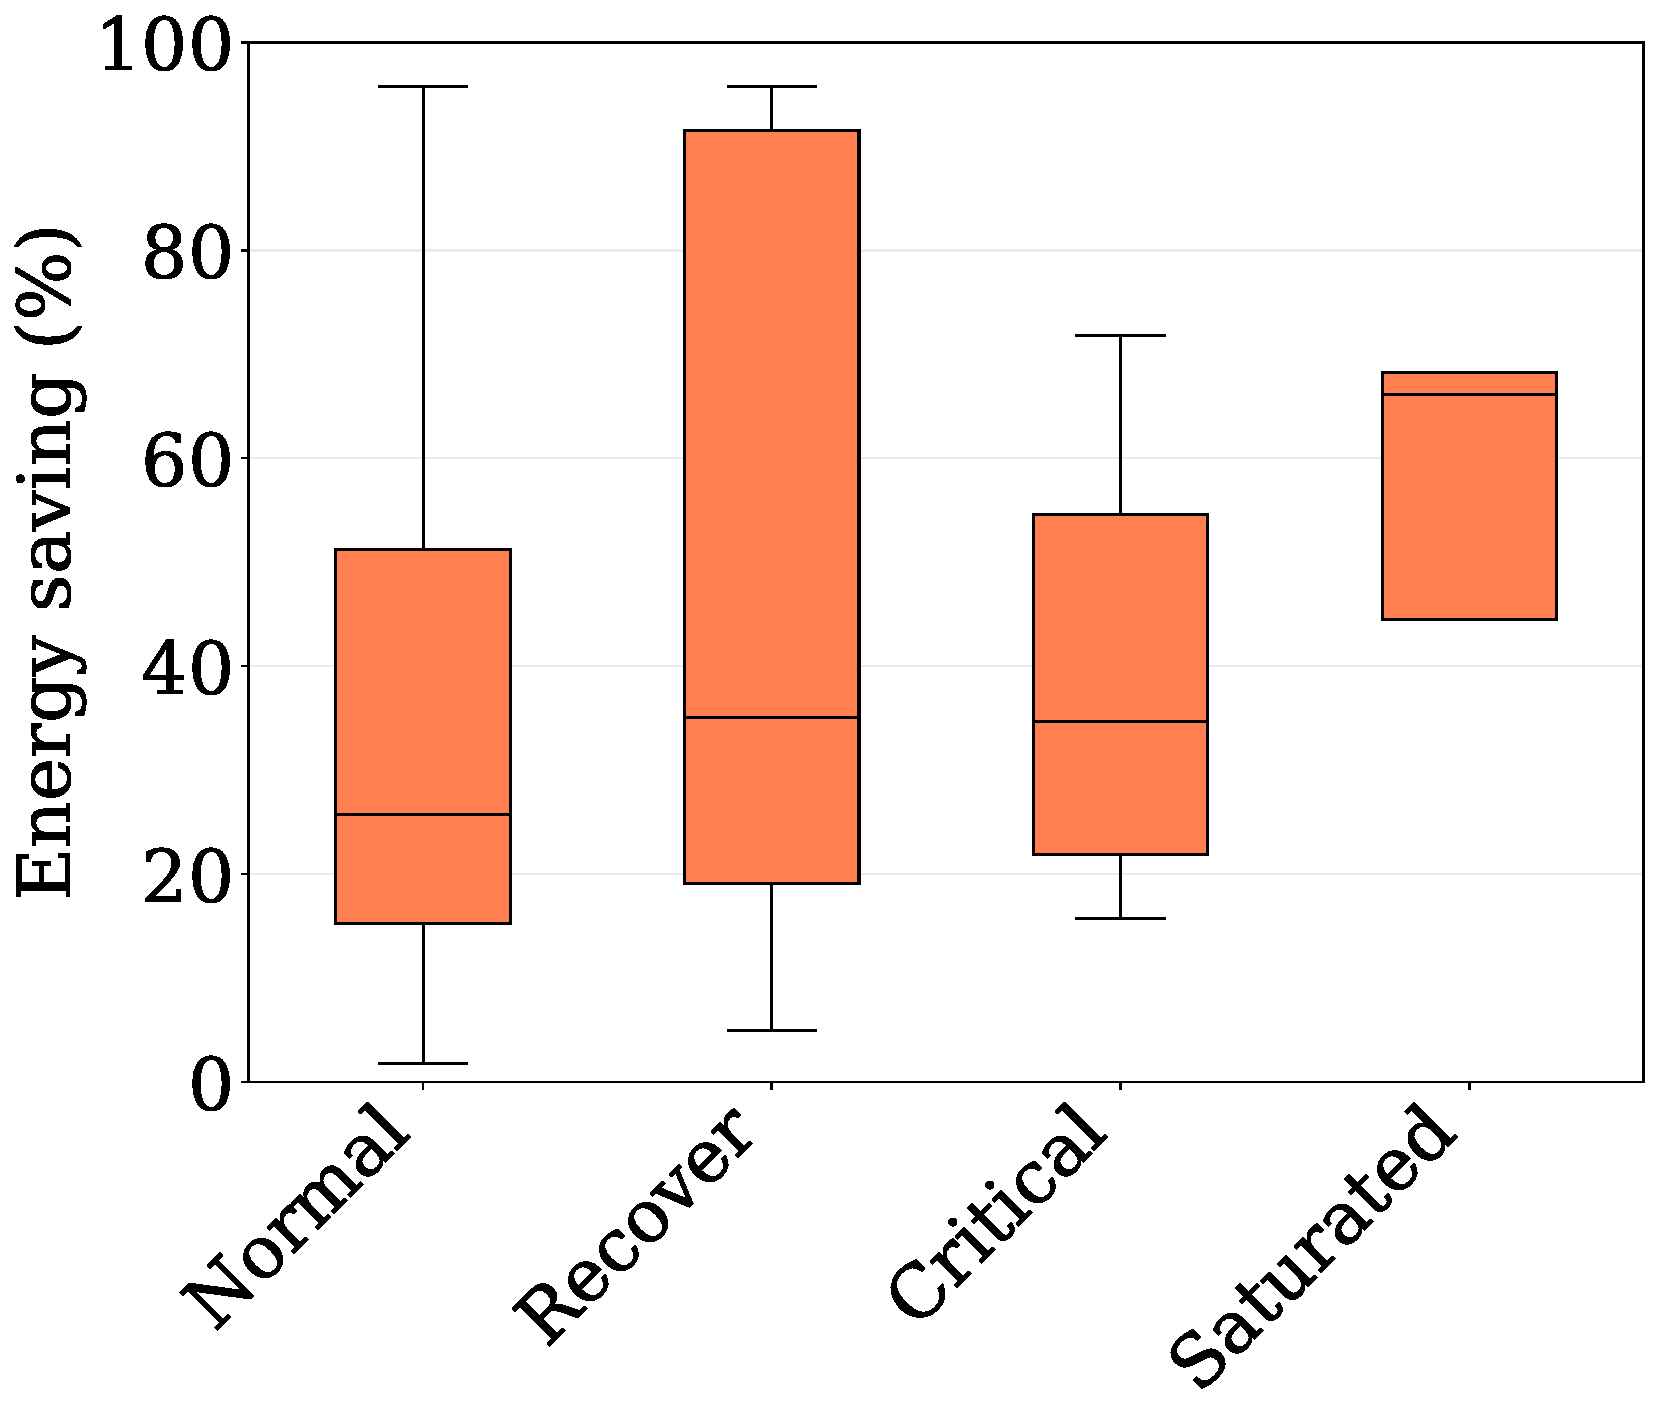
\includegraphics[width=.2\textwidth,trim={0 160pt 0 0},clip]{images/kpi/saving_per_class/north_london/energy_saving_class_24x7_2.pdf}}
    \subfloat{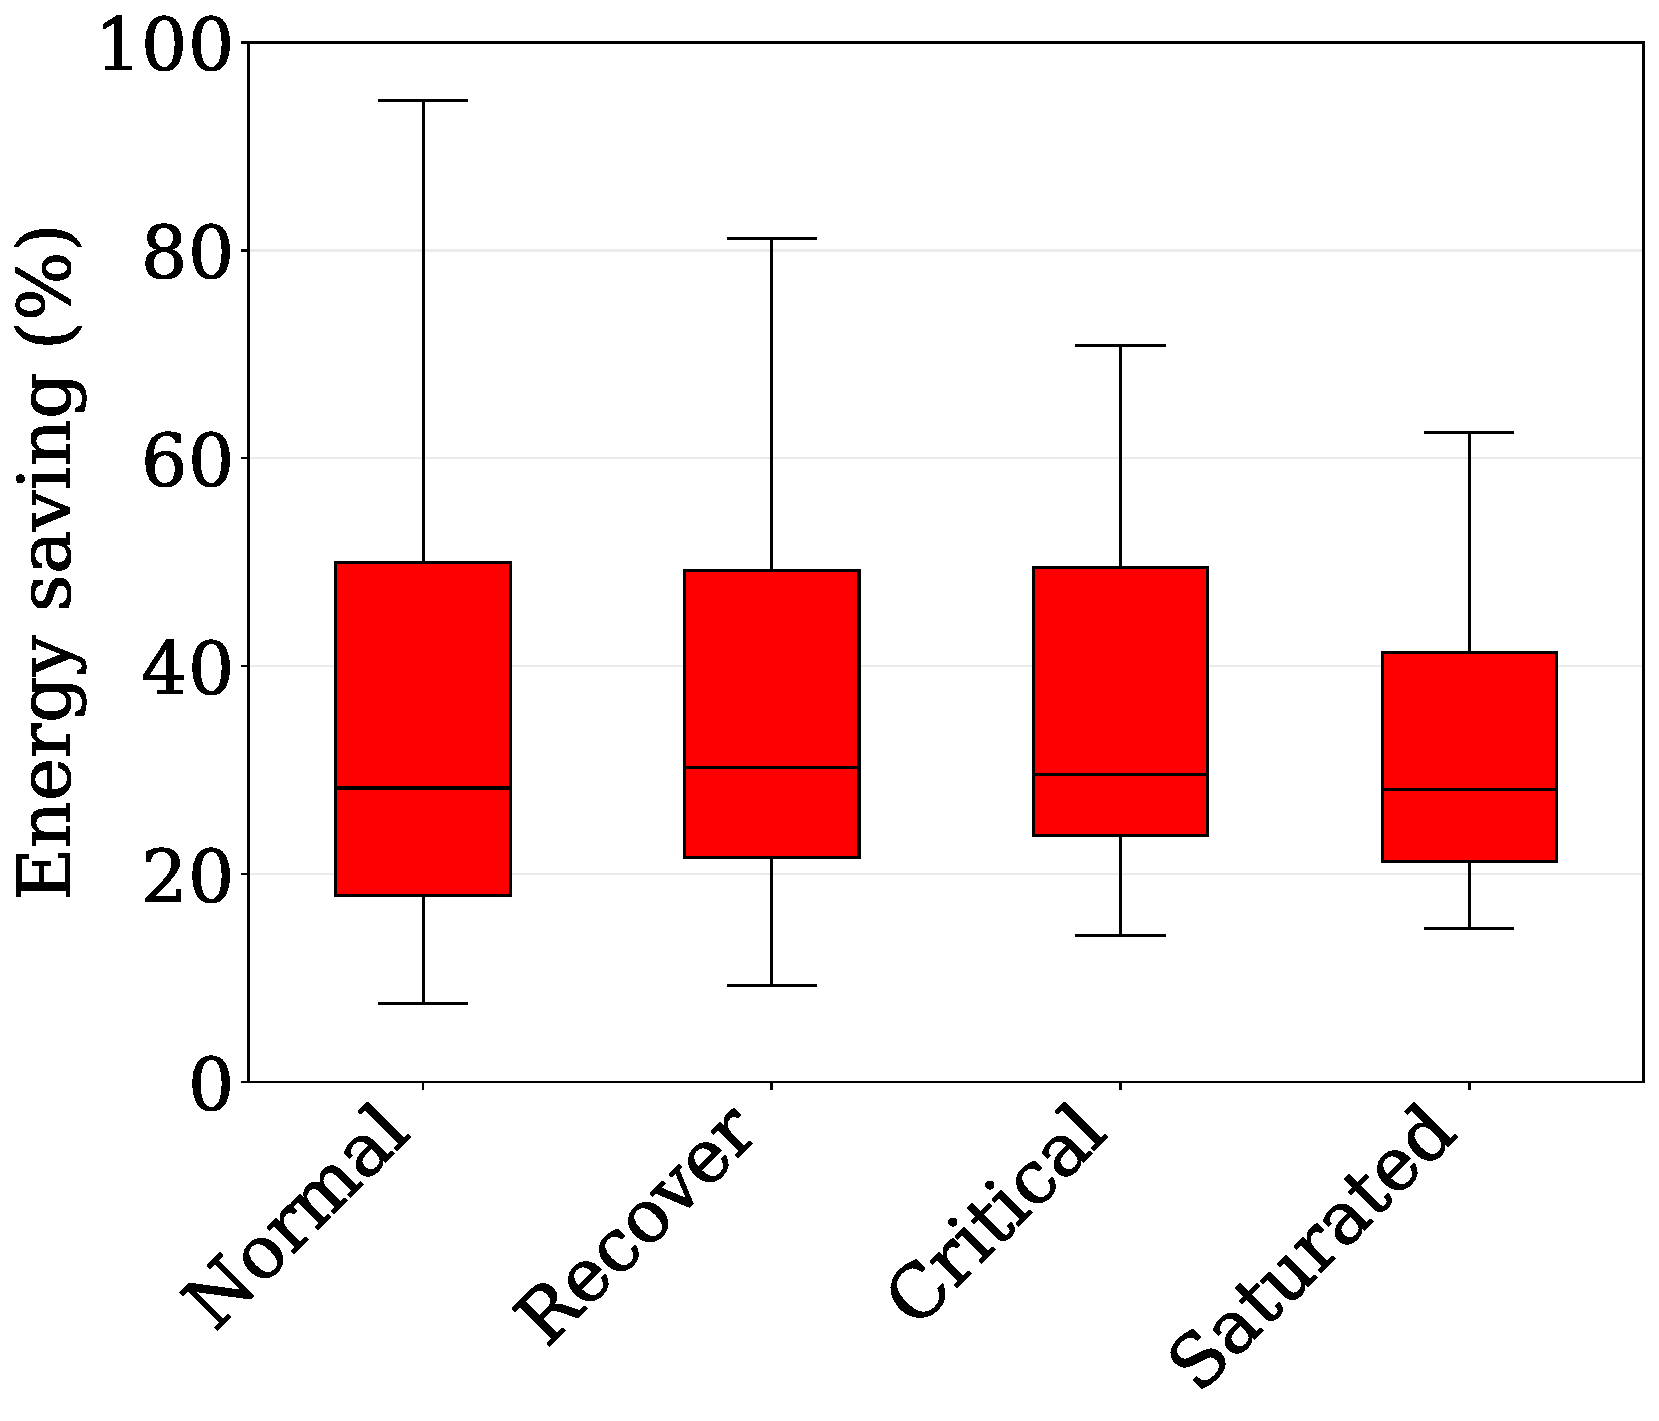
\includegraphics[width=.2\textwidth,trim={0 160pt 0 0},clip]{images/kpi/saving_per_class/north_london/energy_saving_class_24x7_3.pdf}}

    \setcounter{subfigure}{0}
    \subfloat[Night-loose]{
\includegraphics[width=.2\textwidth]{images/kpi/saving_per_class/southeast/energy_saving_class_11_6.pdf}}
    \subfloat[Night-strict]{
\includegraphics[width=.2\textwidth]{images/kpi/saving_per_class/southeast/energy_saving_class_Baseline.pdf}}
    \subfloat[Full-loose]{
\includegraphics[width=.2\textwidth]{images/kpi/saving_per_class/southeast/energy_saving_class_24x7_1.pdf}}
    \subfloat[Full-moderate]{
\includegraphics[width=.2\textwidth]{images/kpi/saving_per_class/southeast/energy_saving_class_24x7_2.pdf}}
    \subfloat[Full-strict]{
\includegraphics[width=.2\textwidth]{images/kpi/saving_per_class/southeast/energy_saving_class_24x7_3.pdf}}
    \vspace*{-4pt}
    \caption{\small Energy consumption saving in each transition class for each energy saving strategy. Top - Dense region, bottom - Sparse region.
    \label{fig:energy_saving_impact_kpi_class}
    }
    \vspace{-10pt}
\end{figure*}

When breaking down energy savings at the level of individual capacity cells, we find a very heterogeneous behavior.
Figure~\ref{fig:energy_saving_impact_kpi_class} shows the energy saving distribution of the capacity cells: there is high variability among the savings, especially with more aggressive policies, in all four cases. This implies that \textit{the same energy saving strategies may be extremely good or bad, depending on the considered cell}. For instance, even a Full-loose policy can be very bad for some cell that saves just $5\%$ of energy, and cause severe saturation every time they enter into sleep mode. Conversely, a Full-strict strategy can work extremely well at some cells, with savings of $60\%$, that have no impact on the end-user.